\begin{answer}
	In order to make GDA perform better on data set 1, we need to re-scale the $x_2$ of valid set to fit the scale of $x_1$ of the valid set and the distribution of $x_1$ of the valid set.
	
	So, I used $x_2 \Leftarrow log(|x_2|)$ to make $x_2$ to fit the $x_1$'s scale and distribution. 
	
	By observing the plot of the change in $x_2$, the performance of GDA on data set 1 slightly improved. 
    \begin{figure*}[h]
        \centering
        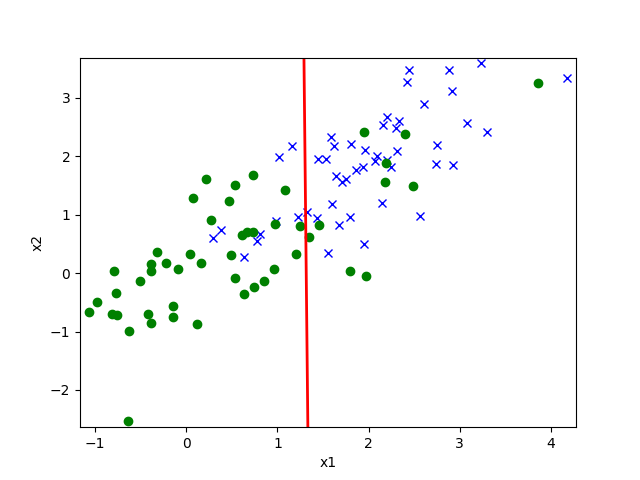
\includegraphics[width=1.0\linewidth]{tex/linearclass/improved_gda_pred_1.png}
        \caption{Plot of improved GDA on data set 1 by changing $x_2$ into $log(|x_2|)$}
        \label{fig:my_label}
    \end{figure*}
	
	
\end{answer}
